\capitulo{3}{Conceptos teóricos}

En esta sección vamos a explicar los algoritmos utilizados en el desarrollo del proyecto. Primero veremos los algoritmos relativos a la planificación de la ruta, y a continuación aquellos relativos al seguimiento de la misma de una forma autónoma por parte del vehículo.

\section{Algoritmo A*}

A* es un algoritmo de búsqueda informada del tipo primero el mejor, que usa una función de evaluación para elegir hacia que nodo expandirse desde un nodo inicial hacia un nodo final.

Para representar el espacio de búsqueda del algoritmo, se usa una cuadrícula, es por lo tanto un algoritmo que opera en un espacio de estados discreto. Cada nodo de la cuadricula puede representar un espacio donde es posible desplazarse o un obstáculo que es inalcanzable.

La función F() de evaluación calcula el coste de cada nodo, con lo que se eligen los nodos con menor coste para llegar al destino a través del camino óptimo. Esta función está formada por dos funciones a su vez: una función G() que calcula el coste del camino seguido desde el nodo inicial a ese nodo concreto, y una función H() o función heurística que hace un estimación del coste del camino desde ese nodo al nodo final o meta.

Al algoritmo comienza desde el nodo inicial explorando los nodos adyacentes o sucesores, cual es de menor coste. Un nodo ya explorado, es decir del que ya se ha buscado sus sucesores, se manda a la lista de nodos cerrados. Con los sucesores se forma una lista de nodos abiertos o por explorar, de la cual se elige el de menor coste para ser el siguiente en ser explorado, hasta que se alcance el nodo meta o no queden más nodos por ser explorados (si no quedasen más nodos significaría que no hay un camino entre el nodo inicial y la meta). Si al explorar un nodo esta ya se encontraba en alguna de las listas de nodos abiertos o cerrados, se actualizarán los valores de los nodos al de menor coste encontrado.

\subsubsection{Heurística}
Al algoritmo A* es completo, lo que significa que encontrará un camino hasta la meta siempre que este exista. Además, para que sea admisible, que significa que siempre encontrará un camino óptimo, su función H() también debe ser admisible.

Una función H() es admisible siempre y cuando no sobrestime el coste del camino desde un nodo hasta la meta. Por ejemplo se puede considerar que el camino desde un nodo hasta la meta será la línea recta.

La admisibilidad del A* trae consigo un gran coste computacional debido al gran número de nodos explorados. Para mejorar la eficiencia podemos dar pesos a las funciones G() y H(), de tal forma que si damos mas valor a G() la búsqueda se expandirá en anchura buscando el camino, mientras que si damos más valor a H() se expandirá más rápido acercándose a la meta.

\subsection{Pseudocódigo A*}

Además de secciones tenemos subsecciones.

\section{\textit{Path Smoothing} o Suavizado}
\textcolor{blue}{Poner imagenes comparativas}

Un problema del A* tradicional es que las rutas que encuentra, aunque sean las más cortas no tienen una apariencia realista. Esto es debido a que el A* discretiza el espacio de búsqueda, en nuestro caso el espacio en tres dimensiones, para poder buscar la ruta. Dependiendo de la representación que elijamos, se acercará más a o menos a la realidad, pero en cualquier caso se producirá una diferencia que suele estar alejada de la representación ideal de esa misma ruta.

Por ejemplo, en el caso de una búsqueda en un parrilla, si seguimos el camino a través de cada casilla, cuando el camino siga una ruta en diagonal, el A* seguirá un camino en zigzag. Aunque este camino es perfectamente válido, en la realidad no se sigue un camino en zigzag sino que se sigue la línea recta que representa. En el caso de las curvas el problema es parecido. El camino encontrado estará formado por segmentos rectos en vez de seguir una ruta redondeada.

Por este motivo una vez realiza una vez obtenida la ruta, un proceso de suavizado de tal forma que se acerque la ruta obtenida a través del A*, a la representación ideal de esa ruta.

\subsection{Eliminar el zigzag}
\textcolor{blue}{Poner imagenes}

El primer método que hemos usado y que suele dar buenos resultados, es eliminar el zigzag. Este método es básicamente lo mismo que realiza el theta* que explicaremos más adelante en \ref{referenciaTheta}.

El zigzag es el problema más habitual que nos hemos encontrado. Al representar un espacio de tres dimensiones a través de casillas, se produce habitualmente porque aunque se use la representación octal permitiendo el movimiento diagonal, esto al pasarlo a un espacio en tres dimensiones quiere decir que sólo tenemos ocho posibles ángulos de movimiento: 0º, 45º, 90º, 135º, 180º, 225º, 270º y 315º

En realidad las posibilidades reales para movernos son cualquier angulo de los 360º. Por tanto, si nuestro objetivo está en un angulo diferente a esos ocho, se produce un zigzag combinándoles hasta que se consigue llegar.

La forma para eliminar el zigzag, es comprobar si es posible eliminar estos pasos intermedios. Es decir, si para llegar al objetivo el A* ha usado varias casillas en el espacio discreto, es posible que en un espacio no discreto pudiéramos llegar directamente con un movimiento en un ángulo distinto a los ocho que permite el A*.

Para ello, usamos la línea de visión. Si existe una línea de visión entre una casilla del A* y otra quiere decir que podemos desplazarnos siguiendo una línea recta formada entre esas dos casillas. Con las casillas devueltas por el A*, comprobamos si existe línea de visión entre ellas. Entre casillas consecutivas siempre habrá línea de visión, porque si no, no sería un camino válido, pero puede también haber línea de visión entre las siguientes de forma que haya casillas sobrantes debido al zigzag y a la forma que tiene el A* de buscar el camino.

Así que lo que comprobamos es que existe una línea de visión entre una casilla del A* y la siguiente más lejana posible, y eliminamos a las casillas intermedias. De esta forma obtenemos una línea recta entre esas dos casillas y eliminamos el zigzag producido por las casillas intermedias.

\subsection{Descenso gradiente}
\textcolor{blue}{poner imágenes con resultados de distintos alphas y betas}

El descenso gradiente es un algoritmo iterativo de optimización que a partir de $N$ valores iniciales ($x_1, x_2, x_3, ..., x_n$), itera una función modificando esos valores gradualmente hacía un mínimo de una función $f(x_1, x_2, x_3, ..., x_n)$. El algoritmo termina cuando el cambio que se producen en los valores es menor que la tolerancia indicada.

Para optimizar la ruta, queremos obtener los valores que minimizan las distancia entre los puntos sucesivos de la ruta, y a su vez que minimicen las distancia a la ruta original.

Para minimizar la distancia entre los puntos con respecto a la ruta original usaremos las función:
\begin{center}
$y_i = y_i + \alpha (x_i - y_i)$
\end{center}
Donde $\alpha$ es el peso que le damos a cuanto de cerca queremos que la ruta suavizada esté de la ruta original, $x$ es el punto de la ruta original e $y$ es el nuevo punto suavizado.

Para minimizar la distancia entre los puntos sucesivos de la ruta, usamos la función:
\begin{center}
$y_i = y_i + \beta (y_{i+1} + y_{i-1} - 2 * y_i)$
\end{center}
Donde $\beta$ es el peso que le damos al suavizado de la ruta, y tenemos en cuenta la distancia tanto con el punto anterior como con el puto siguiente.

Para calcular el error que se produce, o el cambio hacia el mínimo, usamos la función:
\begin{center}
$error = error + (z_i - y_i)$
\end{center}
Donde $z$ es el valor de $y$ antes de calcular el nuevo mínimo.

\subsection{Curvas Bézier}
Las curvas Bézier \cite{bezierdevmag, wiki:bezier} son una forma de representar curvas a través de una función que recibe un parámetro. Hemos usado la función de las curvas de Bézier para suavizar la ruta y así obtener giros y curvas más cercanas a una representación real

Una función de una curva Bézier tiene varios puntos de control (al menos dos). De estos puntos, el primero y el último representan el inicio y el final de la curva. Esta función además recibe un parámetro que puede tomar los valores comprendidos entre cero y uno. Si el parámetro toma el valor cero, entonces la función devuelve el punto de inicio, mientras que si toma el valor uno devuelve el punto final. De esta forma, dando valores entre cero y uno, la función devuelve los valores que se encuentran entre los puntos de inicio y de fin.

Si la función toma dos puntos de referencia, lo que obtendremos sera una recta y sus puntos intermedios. Si la función toma tres puntos entonces tendremos una curva donde el vértice será cercano al punto intermedio. Podemos usar más puntos para representar curvas más complejas o dar curvas con más variedad de formas.

\begin{figure}[htpb]
    \centering
    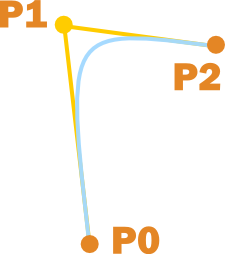
\includegraphics[width=\textwidth,height=6cm,keepaspectratio=true]{bezier_2_devmag}
    \caption[Esquema de una curva Bézier cuadrática de Herman Tulleken]{Esquema de una curva Bézier cuadrática de Herman Tulleken, Bézier Curves for your Games: A Tutorial \cite{bezierdevmag_imagen}.}
    \label{fig:basics AFM sketch}
\end{figure}

Hemos usado la función Bézier con tres puntos después de eliminar el zigzag, así que cada tres puntos del A* sin zigzag se usan como puntos de control que servirán para crear la curva. Si los puntos más o menos están alineados, el resultado será una recta suavizada, y si forman una curva, se eliminan los segmentos rectos y se reemplazan con puntos que forman una curva. 

La función Bézier cuadrática para tres puntos de control y parámetro t es:

\begin{center}
$[x, y, z] = (1 – t)^2P_0 + 2(1 – t)tP_1 + t^2P_2$
\end{center}

En formato expandido:
\begin{center}
$x = (1 – t)^2x_0 + 2(1 – t)tx_1 + t^2x_2$

$y = (1 – t)^2y_0 + 2(1 – t)ty_1 + t^2y_2$

$z = (1 – t)^2z_0 + 2(1 – t)tz_1 + t^2z_2$
\end{center}

\begin{figure}[htpb]
    \centering
    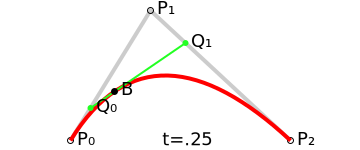
\includegraphics[width=\textwidth,height=6cm,keepaspectratio=true]{Bezier_2_wikipedia}
    \caption[Esquema de una curva Bézier cuadrática, Wikipedia]{Esquema de una curva Bézier cuadrática de Bézier curve --- Wikipedia \cite{wiki:bezierimagen}.}
    \label{fig:basics AFM sketch}
\end{figure}

\newpage

\section{Theta*} \label{referenciaTheta}
Theta A* es un algoritmo desarrollado por A. Nash, K. Daniel, S. Koenig y A. Felner \cite{thetaestrella, thetaestrellaweb} en 2010 que modifica el A* original para obtener rutas más realistas.

Como explicamos anteriormente, el A* por la forma en la que representa el espacio de búsqueda da resultados poco realistas, con lo que hay que realizar un postprocesado de la ruta obtenida. El theta* incorpora este proceso al propio A* para obtener de forma directa rutas que no requieran del proceso de suavizado o que lo minimice.

Para ello, el cambio que hace el Theta* respecto al A* es que un sucesor a una casilla puede ser cualquier casilla, en vez de ser unicamente las que tiene alrededor. El algoritmo es el mismo que el A* original, pero cuando se calculan los sucesores, además de calcular si es un sucesor válido y el coste de ese sucesor, comprueba si hay linea de visión con la casilla del nodo padre del nodo que lo generó. Si no hay línea de visión, sigue el algoritmo del A* y le asigna al sucesor como padre la casilla que lo originó. Pero si hay línea de visión, le asigna como padre no el nodo que lo generó, sino el padre de este, calculando el coste del sucesor teniendo en cuenta esta otra casilla. De esta forma elimina las casillas intermedias que origina el A* que no son necesarias de forma similar a como se realizaría en el post procesado para eliminar el zigzag.

Podemos observar el funcionamiento del algoritmo en la figura 3.3. La línea discontinua roja muestra el camino encontrado por el A*. En cambio, el Theta*, al haber una línea de visión entre el nodo $S_{start}$ y el nodo $S'$, le asigna como padre al nodo $S'$ el nodo $S_{start}$ sin pasar por el nodo intermedio $S$ como hace el A*.

\begin{figure}[htpb]
    \centering
    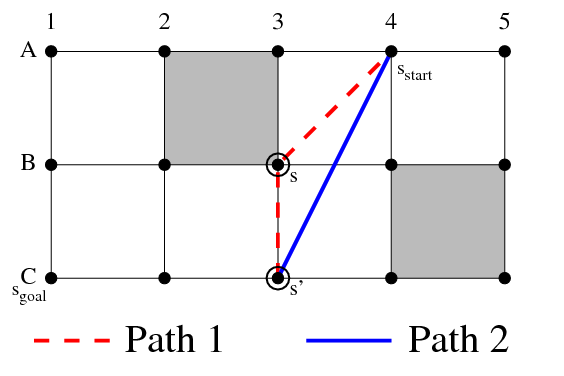
\includegraphics[width=\textwidth,height=6cm,keepaspectratio=true]{Theta_path_12}
    \caption[Comparación de los caminos elegidos por el A* y el Theta*]{Comparación de los caminos elegidos por el A* (path1) y el theta* (path2) de \cite{thetaestrellawebimagen}.}
    \label{fig:basics AFM sketch}
\end{figure}

\subsection{Pseudocódigo Theta*}

\newpage

\section{A* con vértices}
El algoritmo A* como hemos visto, divide el espacio de búsqueda en casillas de un espacio discreto. Esto presenta los problemas de rutas poco realistas, y además al ser discreto, no podemos representar una línea recta entre dos puntos distantes, si no que debemos recorrer todas las casillas intermedias.

Podemos mejorar ambos problemas usando un \textit{Nav Mesh} \ref{referenciaNavMesh}.  Un \textit{Nav Mesh} usa polígonos para representar el espacio de búsqueda de tal forma que los lados de estos polígonos y sus vértices se encuentran en los bordes del espacio recorrible. De esta forma, podemos usar esos vértices como las casillas del espacio discreto, lo que produce tres mejoras importantes:

\begin{enumerate}
\item La representación del espacio recorrible se ajusta más a un espacio continuo al poder ir de un vértice a otro sin pasar por estados intermedios.
\item Permite que las rutas obtenidas sean más realistas que las obtenidas con la representación discreta.
\item Al ser un espacio continuo dentro de los polígonos del \textit{Nav Mesh}, evitamos pasar por todos los estados intermedios de una representación discreta, reduciendo enormemente las casillas a explorar y reduciendo el tiempo de ejecución del algoritmo.
\end{enumerate}

\textcolor{green}{NOTA: no se que mas comentar}

\section{\textit{Hybrid A*}}
Los algoritmos que hemos visto anteriormente, tanto los que usan una representación totalmente discreta hasta los que buscan aproximarse a rutas más realistas en un espacio continúo, tienen el problema de que no tienen en cuenta las características del vehículo que va a realizar la ruta.

El \textit{Hybrid A*} se basa en el A* tradicional, pero teniendo en cuenta estos dos factores: que el vehículo se mueve por un espacio continuo, y que lo hace siguiendo sus limitaciones físicas.

Para ello, utiliza una aproximación continua al A*. En nuestro caso, la aproximación usada ha sido el modelo de la bicicleta. Este modelo es válido porque los ejes de un vehículo son simétricos, por lo que el resultado de un lado del vehículo será equivalente al del otro lado, pudiéndolo simplificar como si fuera un solo eje formado por la rueda delantera y la rueda trasera.

\textcolor{green}{Cual es la referencia correcta a Sebastian Thrun?}
\textcolor{blue}{insertar imagen del modelo de la bicicleta}

Los elementos de este modelo son:
\begin{enumerate}
\item La rotación del vehículo $\theta$.
\item El ángulo de giro de las ruedas $\alpha$
\item La distancia entre los ejes $l$
\item La distancia recorrida por el vehículo $d$
\end{enumerate}

Con estos elementos podemos calcular en que posición se encontrará el vehículo en un espacio de tiempo, teniendo en cuenta su capacidad de maniobra.

Las formulas para el calculo de la nueva posición del vehículo son:
\begin{center}
$x' = x +  v \Delta t sin \theta$

$z' = z +  v \Delta t cos \theta$

$\theta' = \theta + \Delta t \omega $
\end{center}

\textcolor{green}{No se cual sería la formula para la y}

Para $v \Delta t$ hemos realizado una aproximación, tal que hemos considerado que la velocidad del vehículo $v$ va a ser constante, y que $\Delta t$ es el tiempo que tarda en recorrer una unidad de nuestra representación. Esto es válido en nuestro caso y nos permite simplificar las ecuaciones porque la velocidad de nuestro vehículo a través del \textit{PID Control} va a ser aproximadamente constante. En un entorno real $v$ sería la velocidad del vehículo entre el lapso de tiempo recorrido entre las mediciones representado por $\Delta T$ 

Para calcular $\omega$, que es el radio de giro que realiza el vehículo en ese espacio de tiempo continuo, usamos la siguiente fórmula:
\textcolor{green}{referencia de https://www.youtube.com/watch?v=5lWj1FMkq5I  https://www.udacity.com/course/intro-to-artificial-intelligence--cs271 Norvig y thrun}
\begin{center}
$\omega = \displaystyle \frac{d}{l} * tan \alpha  $
\end{center}

Con estos elementos ya podemos calcular cual es el siguiente estado del vehículo en un espacio continuo. Los sucesores del estado actual serán esos estados continuos, variando el angulo de giro, y podemos tener en cuenta el sentido permitiendo al vehículo ir marcha atrás añadiendo los sucesores correspondientes.

Esto nos permite además de obtener rutas más realistas, rutas que se adecuan a la maniobrabilidad del vehículo,  rutas que permiten maniobrar y cambiar de sentido si fuera necesario.

Una de las desventajas del \textit{Hybrid A*} es que no es un algoritmo completo al contrario que el A*. Cuando calculamos los sucesores de un estado se asigna el mejor a una casilla discreta correspondiente del espacio discreto. Además, de forma tradicional el \textit{Hybrid A*} si vuelve a una casilla ya explorada, descarta ese camino. De esta forma, aunque en la mayoría de los casos encontrará un camino, no siempre lo hará aunque exista.

\section{\textit{PID Control}}

\newpage

\section{Comparativa de los algoritmos}
En esta sección vamos a comparar los algoritmos dependiendo de si utilizan una representación del espacio de búsqueda continua o discreta. A continuación también compararemos el rendimiento de los distintos algoritmo tomando como referencia al A*.

\textcolor{green}{coloca las tablas donde no es no se porque}

\tablaSmall{Comparación de los algoritmos según su representación}{l c c }{comparativadiscretocontinuo}
{ \multicolumn{1}{l}{Algoritmo} & Discreto & Continuo \\}{ 
A* & X &\\
Theta* & X &\\
A* vértices & & X\\
Hybrid A* & & X\\
}

\textcolor{blue}{poner valores reales}
\tablaSmall{Comparación de los algoritmos según su rendimiento}{l c c }{comparativarendimiento}
{ \multicolumn{1}{l}{Algoritmo} & Segundos & Porcentaje \\}{ 
A* & 10.0 & 100\%\\
Theta* & 9.0 & 90\%\\
A* vértices & 1.0 & 1\%\\
Hybrid A* & 15 & 150\%\\
}



\section{Imágenes}

Se pueden incluir imágenes con los comandos standard de \LaTeX, pero esta plantilla dispone de comandos propios como por ejemplo el siguiente:

\imagen{escudoInfor}{Autómata para una expresión vacía}



\section{Listas de items}

Existen tres posibilidades:

\begin{itemize}
	\item primer item.
	\item segundo item.
\end{itemize}

\begin{enumerate}
	\item primer item.
	\item segundo item.
\end{enumerate}

\begin{description}
	\item[Primer item] más información sobre el primer item.
	\item[Segundo item] más información sobre el segundo item.
\end{description}
	
\begin{itemize}
\item 
\end{itemize}

\section{Tablas}

Igualmente se pueden usar los comandos específicos de \LaTeX o bien usar alguno de los comandos de la plantilla.

\tablaSmall{Herramientas y tecnologías utilizadas en cada parte del proyecto}{l c c c c}{herramientasportipodeuso}
{ \multicolumn{1}{l}{Herramientas} & App AngularJS & API REST & BD & Memoria \\}{ 
HTML5 & X & & &\\
CSS3 & X & & &\\
BOOTSTRAP & X & & &\\
JavaScript & X & & &\\
AngularJS & X & & &\\
Bower & X & & &\\
PHP & & X & &\\
Karma + Jasmine & X & & &\\
Slim framework & & X & &\\
Idiorm & & X & &\\
Composer & & X & &\\
JSON & X & X & &\\
PhpStorm & X & X & &\\
MySQL & & & X &\\
PhpMyAdmin & & & X &\\
Git + BitBucket & X & X & X & X\\
Mik\TeX{} & & & & X\\
\TeX{}Maker & & & & X\\
Astah & & & & X\\
Balsamiq Mockups & X & & &\\
VersionOne & X & X & X & X\\
} 

\tablaSmall{Herramientas 0}{l c c c c}{herramientasportipodeuso}
{ \multicolumn{1}{l}{Herramientas} & App AngularJS & API REST & BD & Memoria \\}{ 
HTML5 & X & & &\\
CSS3 & X & & &\\
BOOTSTRAP & X & & &\\
JavaScript & X & & &\\
AngularJS & X & & &\\
Bower & X & & &\\
PHP & & X & &\\
Karma + Jasmine & X & & &\\
Slim framework & & X & &\\
Idiorm & & X & &\\
Composer & & X & &\\
JSON & X & X & &\\
PhpStorm & X & X & &\\
MySQL & & & X &\\
PhpMyAdmin & & & X &\\
Git + BitBucket & X & X & X & X\\
Mik\TeX{} & & & & X\\
\TeX{}Maker & & & & X\\
Astah & & & & X\\
Balsamiq Mockups & X & & &\\
VersionOne & X & X & X & X\\
} 
